\documentclass[letterpaper, 10 pt, conference]{ieeeconf}


\usepackage[colorlinks=true, urlcolor=blue, pdfborder={0 0 0}]{hyperref}
\usepackage{xcolor}
\usepackage{amsmath}
\usepackage{geometry}
\usepackage{overpic}
\usepackage{fancyhdr}
\usepackage{url}
\usepackage{graphicx}
\usepackage[caption=false,font=footnotesize]{subfig}

\usepackage{fourier}
\usepackage{amsmath}
\usepackage{pgfplots}

\graphicspath{{./pictures/pdf/},{./pictures/ps/},{./pictures/png/},{./pictures/jpg/}}
\begin{document}
\author{Shiva Shahrokhi, Aaron T. Becker}
\title{Open-Loop Controller}
\maketitle
\thispagestyle{fancy}
\pagestyle{fancy}
\addtolength{\headsep}{0.2in}
\addtolength{\topmargin}{-0.2in}
\lhead{\small pdf at \href{https://github.com/aabecker/SwarmControlSandbox/tree/master/papers/shiva}{github.com/aabecker/SwarmControlSandbox}}

\begin{abstract}
This paper talks about open-loop controller.

\end{abstract}

\section{Open-Loop Mean Controller}




\subsection{Open-Loop Controller for One Robot}

We want to control position and velocity of the robots and deciding about force for reaching our desired position and velocity. So our input is going to be accelerator(\emph{F = ma}). If we show acceleration by \emph{a}, velocity by \emph{v} and position in x coordinate by \emph{$P_x$} and in y coordinate by \emph{$P_y$}, we have the following equations
\begin{equation}
\begin{bmatrix}
\dot{P}_x = v_x \\
\dot{v}_x = a_x
\end{bmatrix}
\end{equation}
\begin{equation}
\begin{bmatrix}
\dot{P}_y = v_y \\
\dot{v}_y = a_y
\end{bmatrix}
\end{equation}



The state-space representation of our OpenLoop controller is: 
\begin{align}
\dot{x}(t)  &=  A x(t) + B u(t) \\
y &= C x(t) + D u(t)\nonumber
\end{align}


where \emph{x(t)} represents our states, \emph{u(t)} is our input and \emph{e(t)} represents noise in the system. We also have \emph{y} as our output.\\
First we assume that we don't have noise in the system and we also have just one robot. As mentioned, \emph{a} is our input and \emph{x, y,} and their velocities are our states that we want to control.\\
We define our states as following:
\begin{align}
x_1 &= P_x \\ \nonumber
\dot{x}_1 &= x_2 = \dot{P}_x = v_x\\\nonumber
x_3 &= P_y\\ \nonumber
 \dot{x}_3 &= x_4 = \dot{P}_y = v_y \nonumber
\end{align}


So our state space representation is:
\begin{equation}
\begin{bmatrix}
\dot{x}_1\\ 
\dot{x}_2\\
\dot{x}_3\\
\dot{x}_4
\end{bmatrix} = \begin{bmatrix}
0 & 1 & 0 & 0 \\
0 & 0 & 0 & 0\\
0 & 0 & 0 & 1\\
0 & 0 & 0 & 0
\end{bmatrix}  \begin{bmatrix}
x_1\\
x_2\\
x_3\\
x_4
\end{bmatrix} + \begin{bmatrix}
0 & 0 \\
1 & 0 \\
0 & 0 \\
0 & 1
\end{bmatrix} u
\end{equation}

We want to find number of states that we can control. We need to know rank of the controllability matrix \emph{\{B, AB,$A^2$B, ... , $A^{n-1}$B\}}.
\begin{equation}
C = \{ B, AB, A^2B, ... , A^{n-1}B \}
\end{equation}

\begin{equation}
C=\left\{
\begin{bmatrix} 
0 & 0\\
1 & 0 \\
0 & 0 \\
0 & 1
\end{bmatrix}
,
\begin{bmatrix} 
1 & 0\\
0 & 0\\
0 & 1\\
0 & 0
\end{bmatrix}
\begin{bmatrix} 
0 & 0\\
0 & 0\\
0 & 0\\
0 & 0
\end{bmatrix}
,
\begin{bmatrix} 
0 & 0\\
0 & 0\\
0 & 0\\
0 & 0
\end{bmatrix}
 \right\}
\end{equation}
So we showed that we have two controllable states.


\subsection{Controlling Position for More than One Robot}
We know that we can control velocity of our robot, we want to see what happens if we had more than one robot? As we saw here, $v_x$ is completely independent of $v_y$, so if we wanted to have n robots, we had n states in x axis, and n states in y axis, which were completely independent from each other. So assume we have n robots and want to control them in \emph{x} axis:\\
\begin{align}
\dot{P}_{x1} &= v_{x1}\\\nonumber
\dot{v}_{x1} &= a_{x1}\\\nonumber
\dot{P}_{x2} &= v_{x2}\\\nonumber
\dot{v}_{x2} &= a_{x2}\\\nonumber
&\vdots\\\nonumber
\dot{P}_{xn} &= v_{xn}\\\nonumber
\dot{v}_{xn} &= a_{xn}\nonumber
\end{align}


So our state-space representation will be:
\begin{equation}
\begin{bmatrix}
\dot{x}_1\\ 
\dot{x}_2\\
.\\
.\\
.\\
\dot{x}_{2n-1}\\
\dot{x}_{2n}

\end{bmatrix} = \begin{bmatrix}
0 & 1 & . & . & . & 0 & 0 \\
0 & 0 & . & . & . & 0 & 0 \\
0 & 0 & 0 & 1 & . & 0 & 0 \\
0 & 0 & 0 & 0 & . & 0 & 0 \\
. & . & . & . & . & . & . \\
0 & 0 & . & . & . & 0 & 1 \\
0 & 0 & . & . & . & 0 & 0 
\end{bmatrix}  \begin{bmatrix}
x_1\\
x_2\\
.\\
.\\
.\\
x_{2n-1}\\
x_{2n}
\end{bmatrix} + \begin{bmatrix}
0\\
1\\
.\\
.\\
.\\
0\\
1
\end{bmatrix} a_x
\end{equation}

If we had n robots, we had exactly the same symmetry of what we had for 1 robot. We can again control two states because we have rank two in C:
\begin{equation}
C=\left\{ \begin{bmatrix} 
0\\
1\\
.\\
.\\
.\\
0\\
1
\end{bmatrix}
,
  \begin{bmatrix} 
1\\
0\\
.\\
.\\
.\\
1\\
0
\end{bmatrix}
,
\begin{bmatrix} 
0\\
0\\
.\\
.\\
.\\
0\\
0
\end{bmatrix}, ... \right\}
\end{equation}  
 


\subsection{Controlling Mean Position}
So for any number of robots if we give a global command to them, we have just two controllable states in each axis. So it is obvious that we can not control position of all the robots, but what states are controllable? To answer this question we create a reduced order system that calculates average position and average velocity of the robots:\\

\begin{equation}
\begin{bmatrix}
\dot{\bar{x}}_p \\
\dot{\bar{x}}_v
\end{bmatrix} = \frac{1}{n} \begin{bmatrix}
0& 1& 0& 1& ... &0& 1 \\
0& 0& 0& 0& ... &0& 0
\end{bmatrix}
\begin{bmatrix}
x_1\\
x_2\\
.\\
.\\
.\\
x_{2n-1}\\
x_{2n}
\end{bmatrix} + \frac{1}{n}\begin{bmatrix}
0& 0& 0& 0& ... &0& 0 \\
0& 1& 0& 1& ... &0& 1
\end{bmatrix}\begin{bmatrix} 
0\\
1\\
.\\
.\\
.\\
0\\
1
\end{bmatrix} u_x
\end{equation}
Thus:
\begin{equation}
\begin{bmatrix}
\dot{\bar{x}}_p \\
\dot{\bar{x}}_v
\end{bmatrix} = \begin{bmatrix}
0& 1 \\
0& 0
\end{bmatrix}
\begin{bmatrix}
\bar{x}_p\\
\bar{x}_v
\end{bmatrix} + \begin{bmatrix} 
0\\
1
\end{bmatrix} u
\end{equation}

We analyze \emph{C} for \emph{y}:
\begin{equation}
C=\left\{ \begin{bmatrix} 
0\\
1
\end{bmatrix}
,
 \begin{bmatrix} 
1\\
0
\end{bmatrix}
 \right\}
\end{equation}

This matrix again  has rank two, and thus all the states are controllable. These controllable states are the average position and average velocity:
\begin{equation}
a = K\begin{bmatrix}
\begin{bmatrix}
\dot{\bar{x}}_p \\
\dot{\bar{x}}_v
\end{bmatrix}
-
\begin{bmatrix}
x_{goal} \\
\dot{x}_{goal}
\end{bmatrix}
\end{bmatrix}
\end{equation}
%$\blacksquare$ \\

\subsection{Applying Noise}
Real systems, especially at the micro scale, are affected by unmodelled dynamics much of which can be designed by Brownian noise. To model this equation (3) must be modified as follows:
\begin{align}
\dot{x}(t)  &=  A x(t) + B u(t) + We(t)\\
y &= C x(t) + D u(t)\nonumber
\end{align}
where $e(t)$ is the error in the system.

After some time, gaussian distribution shapes the outline of the robots because of the brownian noise feature:\\
\begin{equation}
P(x) = \frac{1}{{\sigma \sqrt {2\pi } }}e^{{{ - \left( {x - \mu } \right)^2 } \mathord{\left/ {\vphantom {{ - \left( {x - \mu } \right)^2 } {2\sigma ^2 }}} \right. \kern-\nulldelimiterspace} {2\sigma ^2 }}}
\end{equation}

where $\sigma$ is standard deviation:
\begin{equation}
\sigma = \sqrt{\frac{1}{N-1} \sum_{i=1}^N (x_i - \overline{x})^2}
\end{equation}
After a while, if we have lots of robots, we see the robots to make a bell shaped curve because of the Brownian noise. In we see the probability density function of a Gaussian distribution:\\

\begin{equation}
%f(x) \texttildelow N(\mu , \sigma)
\end{equation}
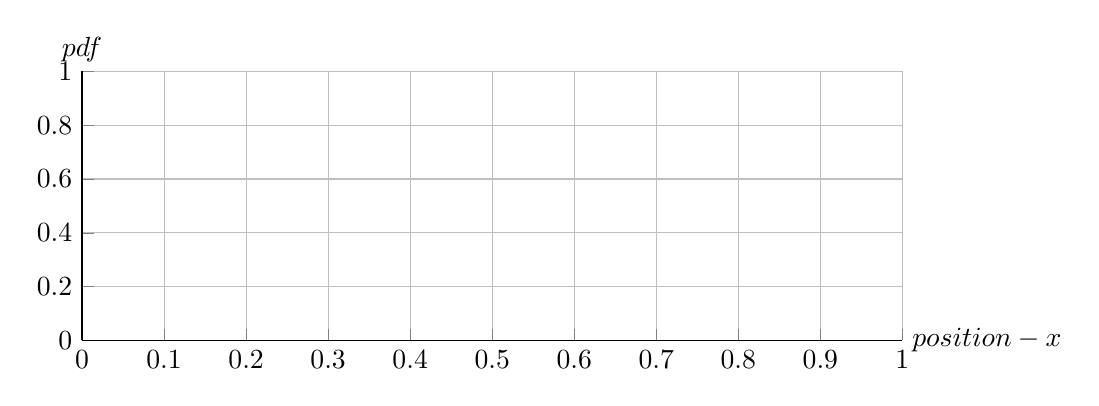
\begin{tikzpicture}
\begin{axis}[
  no markers, domain=-4:4, samples=100,
  axis lines*=left, xlabel=$position-x$, ylabel=$pdf$,
  every axis y label/.style={at=(current axis.above origin),anchor=south},
  every axis x label/.style={at=(current axis.right of origin),anchor=west},
  height=5cm, width=12cm,
  xtick={0}, ytick=\empty,
  enlargelimits=false, clip=false, axis on top,
  grid = major
  ]
  %\addplot [fill=cyan!20, draw=none, domain=-4:1] {gauss(0,1)} \closedcycle;
  %\addplot [fill=cyan!20, draw=none, domain=-4:1] {gauss(0,1)+ gauss(2,1)} \closedcycle;
%  \addplot [fill=cyan!20, draw=none, domain=0:8] {gauss(4,1)} \closedcycle;
%  \addplot [very thick,cyan!50!black , domain= 0:8 ] {gauss(4,1)};
  %\addplot [very thick,cyan!50!black , domain= -4:1] {gauss(2,1)};


%\draw [yshift=-0.6cm, latex-latex](axis cs:-1,0) -- node [fill=white] {Mirrored} (axis cs:1,0);
\end{axis}

\end{tikzpicture}

Probability of the position of the robots, if we have Gaussian noise. \\


If robots face a wall, we expect to have the following shape:\\


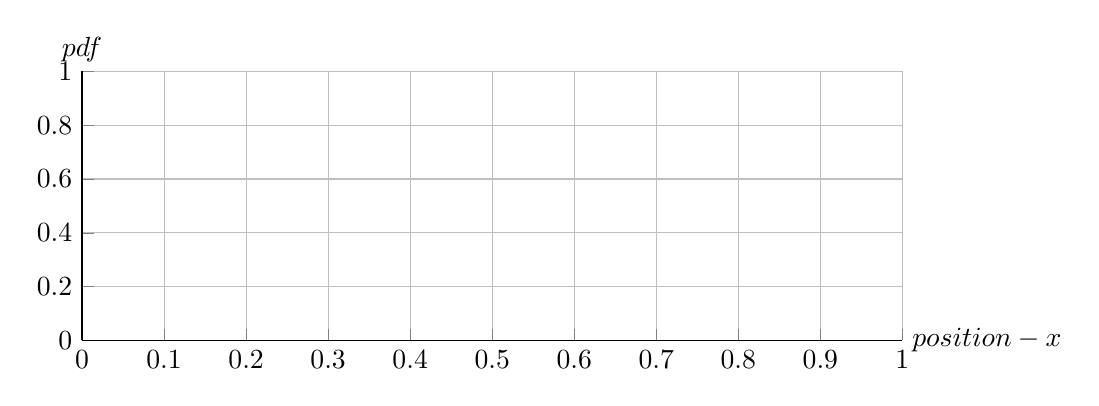
\begin{tikzpicture}
\begin{axis}[
  no markers, domain=-4:4, samples=100,
  axis lines*=left, xlabel=$position-x$, ylabel=$pdf$,
  every axis y label/.style={at=(current axis.above origin),anchor=south},
  every axis x label/.style={at=(current axis.right of origin),anchor=west},
  height=5cm, width=12cm,
  xtick={0,5}, ytick=\empty,
  enlargelimits=false, clip=false, axis on top,
  grid = major
  ]
  %\addplot [fill=cyan!20, draw=none, domain=0:5] {gauss(6,1)} \closedcycle;
%  \addplot [fill=red!20, draw=none, domain=0:5] {gauss(4,1)+ gauss(6,1)} \closedcycle;
  %\addplot [fill=cyan!20, draw=none, domain=-4:4] {gauss(0,2)} \closedcycle;
%  \addplot [very thick,cyan!50!black, domain= 0:8 ] {gauss(4,1)};
%  \addplot [very thick,cyan!50!black , domain= 0:5] {gauss(6,1)};

%\draw [yshift=-0.6cm, latex-latex](axis cs:3,0) -- node [fill=white] {Mirrored} (axis cs:5,0);
\end{axis}

\end{tikzpicture}



 
 \end{document}